\documentclass[landscape]{article}
\usepackage[paperwidth=222mm, paperheight=183mm, margin=0cm]{geometry}
\usepackage{tikz}
\usepackage{xcolor}
\definecolor{myBlue}{RGB}{173, 216, 230}
\definecolor{myGrey}{RGB}{230, 230, 230}
\usetikzlibrary{positioning, shapes.geometric, arrows}
\usepackage{amsmath}

% Define styles
\tikzstyle{node} = [rectangle, rounded corners, minimum width=1.5cm, minimum height=1cm, text centered, draw=black]
\tikzstyle{arrow} = [thick,->,>=stealth]

\begin{document}

\begin{figure}[h]
    \centering
    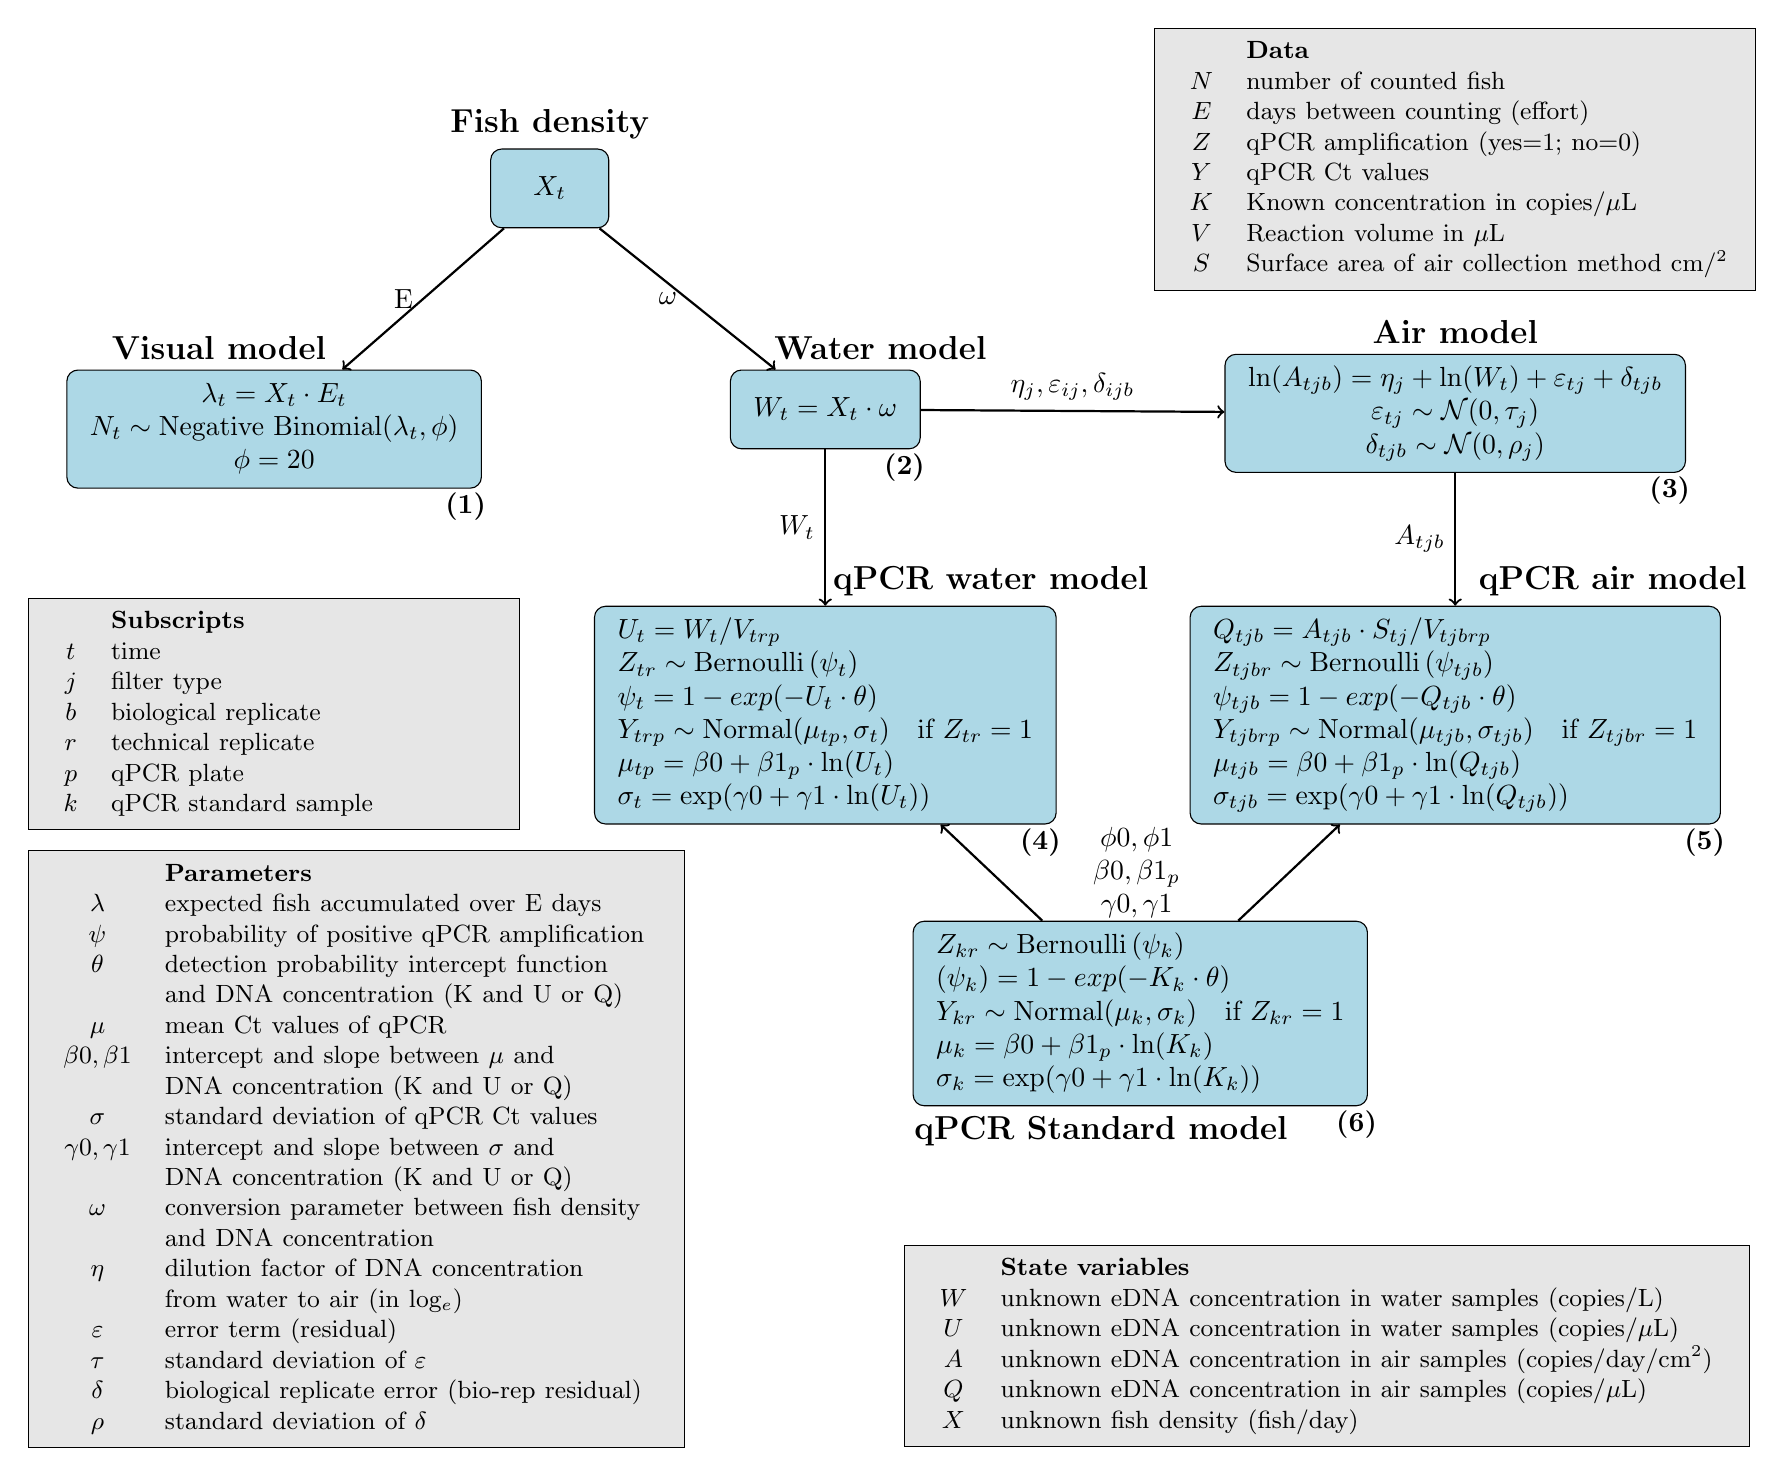
\begin{tikzpicture}[node distance=1.5cm]


%%%%%%%%%%% TRUE FISH %%%%%%%%%%%
\node (Fish_TRUE) [node, fill=myBlue] at (-3.5,0.8) {
    \textbf{$X_t$}
};
\node [above=of Fish_TRUE, yshift=-1.5cm, font=\large\bfseries] {Fish density};

%%%%%%%%%%% Water %%%%%%%%%%%
\node (water) [node, below=of Fish_TRUE, fill=myBlue]  at (0,0) {
    $\begin{array}{c}
        %\lambda_{i} = W_{i} \cdot \omega
        W_{t} = X_t \cdot \omega
        %W_{i} = \lambda_{i} \cdot \omega
    \end{array}$
};
\node [above=of water, xshift=0.7cm, yshift=-1.5cm, font=\large\bfseries] {Water model};
\node[anchor=south east] at ([xshift=5pt, yshift=-15pt] water.south east) {\textbf{(2)}};


%%%%%%%%%%% Air %%%%%%%%%%%
\node (air) [node, below=of Fish_TRUE, fill=myBlue]  at (8,0.20) {
    $\begin{array}{c}
        \ln(A_{tjb}) = \eta_{j} + \ln(W_{t}) + \varepsilon_{tj} + \delta_{tjb} \\
        \varepsilon_{tj} \sim \mathcal{N}(0,\tau_j) \\
        \delta_{tjb} \sim \mathcal{N}(0,\rho_j)
        %\ln(A_{ij}) = \ln(A_{ijb}) + \delta_{b} \\
        %\ln(A_{ij}) = \eta_{j} + \ln(W_{i}) + \varepsilon_{ij} \vspace{3px}\\
        %A_{ij} = \frac{1}{B} \cdot \sum_{b=1}^{B} A_{ijb} \vspace{3px}\\
        %\delta_{b} = A_{ij} - A_{ijb} \\
    \end{array}$
};
\node [above=of air, yshift=-1.5cm, font=\large\bfseries] {Air model};
\node[anchor=south east] at ([xshift=5pt, yshift=-15pt] air.south east) {\textbf{(3)}};


%%%%%%%%%%% Visual %%%%%%%%%%%
\node (visual) [node, below=of Fish_TRUE, fill=myBlue]  at (-7,0) {
    $\begin{array}{c}
        %X_i = \lambda_{i} \cdot E_{i}^{-1} \\
        \lambda_{t} = X_t \cdot E_{t} \\
        N_{t} \sim \mathrm{Negative\ Binomial}(\lambda_{t},\phi)\\
        \phi = 20
    \end{array}$
};
\node [above=of visual, xshift=-0.7cm, yshift=-1.5cm, font=\large\bfseries] {Visual model};
\node[anchor=south east] at ([xshift=5pt, yshift=-15pt] visual.south east) {\textbf{(1)}};



%%%%%%%%%%% qPCR env water %%%%%%%%%%%
\node (qPCR_en_wat) [node, below=of water, fill=myBlue]  at (0,-3) {
    $\begin{array}{l}
    U_t = W_t / V_{trp} \\
        Z_{tr} \sim \mathrm{Bernoulli} \left(\psi_{t}\right) \\
        %logit(\psi_{i}) = \phi0 + \phi1 \cdot \ln (W_{i}) \\
        \psi_{t} = 1 - exp(-U_{t} \cdot \theta) \\
        Y_{trp} \sim \mathrm{Normal} (\mu_{tp}, \sigma_{t}) \quad \textnormal{if } Z_{tr} = 1 \\
        \mu_{tp} = \beta0 + \beta1_{p} \cdot \ln (U_{t}) \\
        \sigma_{t} = \exp(\gamma0 + \gamma1 \cdot \ln (U_{t}))
    \end{array}$
};
\node [above=of qPCR_en_wat, xshift=2.1cm, yshift=-1.5cm, font=\large\bfseries] {qPCR water model};
\node[anchor=south east] at ([xshift=5pt, yshift=-15pt] qPCR_en_wat.south east) {\textbf{(4)}};  



%%%%%%%%%%% qPCR env air %%%%%%%%%%%
\node (qPCR_en_air) [node, below=of air, fill=myBlue]  at (8,-3) {
    $\begin{array}{l}
    Q_{tjb} = A_{tjb} \cdot S_{tj} / V_{tjbrp} \\
        Z_{tjbr} \sim \mathrm{Bernoulli} \left(\psi_{tjb}\right) \\
        %logit(\psi_{ijb}) = \phi0 + \phi1 \cdot \ln (Q_{ijb}) \\
        \psi_{tjb} = 1 - exp(-Q_{tjb} \cdot \theta) \\
        Y_{tjbrp} \sim \mathrm{Normal} (\mu_{tjb}, \sigma_{tjb}) \quad \textnormal{if } Z_{tjbr} = 1 \\
        \mu_{tjb} = \beta0 + \beta1_{p} \cdot \ln (Q_{tjb}) \\
        \sigma_{tjb} = \exp(\gamma0 + \gamma1 \cdot \ln (Q_{tjb}))
    \end{array}$
};
\node [above=of qPCR_en_air, xshift=2.0cm, yshift=-1.5cm, font=\large\bfseries] {qPCR air model};
\node[anchor=south east] at ([xshift=5pt, yshift=-15pt] qPCR_en_air.south east) {\textbf{(5)}};  



%%%%%%%%%%% qPCR std water %%%%%%%%%%%
\node (qPCR_st) [node, below=of qPCR_en_wat, fill=myBlue] at (4,-7) {
    $\begin{array}{l}
        Z_{kr} \sim \mathrm{Bernoulli} \left(\psi_{k}\right) \\
        %logit(\psi_{k}) = \phi0 + \phi1 \cdot \ln (K_{k}) \\
        (\psi_{k}) = 1 - exp(-K_{k} \cdot \theta) \\
        Y_{kr} \sim \mathrm{Normal} (\mu_{k}, \sigma_{k}) \quad \textnormal{if } Z_{kr} = 1 \\
        \mu_{k} = \beta0 + \beta1_{p} \cdot \ln (K_{k}) \\
        \sigma_{k} = \exp(\gamma0 + \gamma1 \cdot \ln (K_{k}))
    \end{array}$
};
\node [below=of qPCR_st, xshift=-0.5cm, yshift=1.5cm, font=\large\bfseries] {qPCR Standard model};
\node[anchor=south west] at ([xshift=-15pt, yshift=-15pt] qPCR_st.south east) {\textbf{(6)}};


 % Arrows
        \draw [->, thick] (Fish_TRUE) -- node[midway, left] {E} (visual);
        \draw [->, thick] (Fish_TRUE) -- node[midway, left] {$\omega$} (water);
        \draw [->, thick] (water) -- node[midway, above] {$\eta_j,\varepsilon_{ij},\delta_{ijb}$} (air);
        \draw [<-, thick] (qPCR_en_air) -- node[midway, left] {$A_{tjb}$} (air);
        \draw [<-, thick] (qPCR_en_wat) -- node[midway, left] {$W_t$} (water);

        \draw [->, thick] (qPCR_st) -- node[midway, right, xshift=28pt] {
        $\begin{array}{c}
            \phi0, \phi1 \\ \beta0, \beta1_p \\ \gamma0, \gamma1
        \end{array}$} (qPCR_en_wat);
        \draw [->, thick] (qPCR_st) -- node[midway, right, xshift=8pt] {} (qPCR_en_air);



\node (parameters) [rectangle, draw, 
align=left, right=of qPCR_st, text width=8.1cm, fill=myGrey] at (-11.63,-11.4) {
\small{
      \begin{tabular}{cl}
    &\textbf{Parameters} \\
    $\lambda$ & expected fish accumulated over E days\\
    $\psi$&probability of positive qPCR amplification \\
    $\theta$ & detection probability intercept function\\
    & and DNA concentration (K and U or Q) \\
    $\mu$&mean Ct values of qPCR \\
    $\beta0, \beta1$&intercept and slope between $\mu$ and \\
    &DNA concentration (K and U or Q) \\
    $\sigma$&standard deviation of qPCR Ct values \\
    $\gamma0, \gamma1$&intercept and slope between $\sigma$ and\\
    &DNA concentration (K and U or Q) \\
    $\omega$&conversion parameter between fish density\\
    &and DNA concentration\\
    $\eta$&dilution factor of DNA concentration\\
    &from water to air (in log$_e$)\\
    $\varepsilon$&error term (residual) \\
    $\tau$& standard deviation of $\varepsilon$ \\
    $\delta$&biological replicate error (bio-rep residual)\\
    $\rho$& standard deviation of $\delta$ 
    \end{tabular}
    }
};

% Legend: Subscripts
\node (subscripts) [rectangle, draw, align=left, below=of qPCR_st, text width=6cm, fill=myGrey] at (-7,-2.9) {
\small{
      \begin{tabular}{cl}
    &\textbf{Subscripts} \\
    $t$&time \\
    $j$&filter type \\
    %$j$&sample\\
    $b$&biological replicate\\
    $r$&technical replicate \\
    $p$&qPCR plate \\
    $k$&qPCR standard sample
        \end{tabular}
    }
};

\node (data) [rectangle, draw, align=left, above=of air, text width=7.4cm, fill=myGrey] at (8,-2.0){
\small{
      \begin{tabular}{cl}
    &\textbf{Data} \\
    $N$&number of counted fish \\
    $E$&days between counting (effort)\\
    $Z$&qPCR amplification (yes=1; no=0) \\
    $Y$&qPCR Ct values \\
    $K$&Known concentration in copies/$\mu$L \\
    $V$&Reaction volume in $\mu$L \\
    $S$&Surface area of air collection method cm/$^2$
     \end{tabular}
    }
};

% Legend: State variables
\node (state) [rectangle, draw, align=left, right=of qPCR_st, text width=10.5cm, fill=myGrey] at (-0.5,-13.9){
\small{
      \begin{tabular}{cl}
    &\textbf{State variables} \\
    $W$&unknown eDNA concentration in water samples (copies/L) \\
    $U$&unknown eDNA concentration in water samples (copies/$\mu$L) \\
    $A$&unknown eDNA concentration in air samples (copies/day/cm$^2$)\\
    $Q$&unknown eDNA concentration in air samples (copies/$\mu$L) \\
    $X$&unknown fish density (fish/day) \\
         \end{tabular}
    }
};
    \end{tikzpicture}
    %\caption{Multifish DAG}
\end{figure}

\end{document}
